%%%%%%%%%%%%%%%%%%%%%%%%%%%%%%%%%%%%%%%%%%%%%%%%%%
%
%  New template code for TAMU Theses and Dissertations starting Fall 2012.  
%  For more info about this template or the 
%  TAMU LaTeX User's Group, see http://www.howdy.me/.
%
%  Author: Wendy Lynn Turner 
%	 Version 1.0 
%  Last updated 8/5/2012
%
%%%%%%%%%%%%%%%%%%%%%%%%%%%%%%%%%%%%%%%%%%%%%%%%%%%
%%%%%%%%%%%%%%%%%%%%%%%%%%%%%%%%%%%%%%%%%%%%%%%%%%%%%%%%%%%%%%%%%%%%%%
%%                           SECTION IV
%%%%%%%%%%%%%%%%%%%%%%%%%%%%%%%%%%%%%%%%%%%%%%%%%%%%%%%%%%%%%%%%%%%%%

\chapter{\uppercase{Seismic Data Analytics Platform}}

In oil \& gas companies, the data analytics software is not only used by scientists and researchers, but also the employees who do not have the background of computer science. To allow those users to browse the seismic data and to generate analytics result, we developed some user-friendly utilities on top of Seismic Data Analytics SDK to simplify the way for deploying general purpose applications on Spark-Hadoop platform, which include a distributed data server for remote data access, the web interfaces for remote data visualization and user-defined workflow. With these tools, the users, not only the developers, are able to easily facilitate their works with this Seismic Data Analytics Platform in minimal efforts.


\section{Data Server and Remote Web Visualization}

In petroleum industry, an important application scenario is data visualization, which allows user to browse and analyze seismology features of seismic data in 3D spacing. With visualization tools, computer renders the seismic data to 3D graphic views and allows user to browse and manipulate the graph along any direction, which inspired the geophysicists and data scientists to develop various of useful models. However,traditional visualization tools in industry are only capable of handling small datasets, or render only few segments of the big datasets at a time. The performance of  big dataset visualization has long been the critical bottleneck of regular workflow of industry.

To resolve this problem, we developed a web-based remote data visualization service which is able to load and render the seismic data for 3D visualization in real-time. Figure \ref{visualization_framework} shows the framework of this service. 

\begin{figure}[h]
\centering
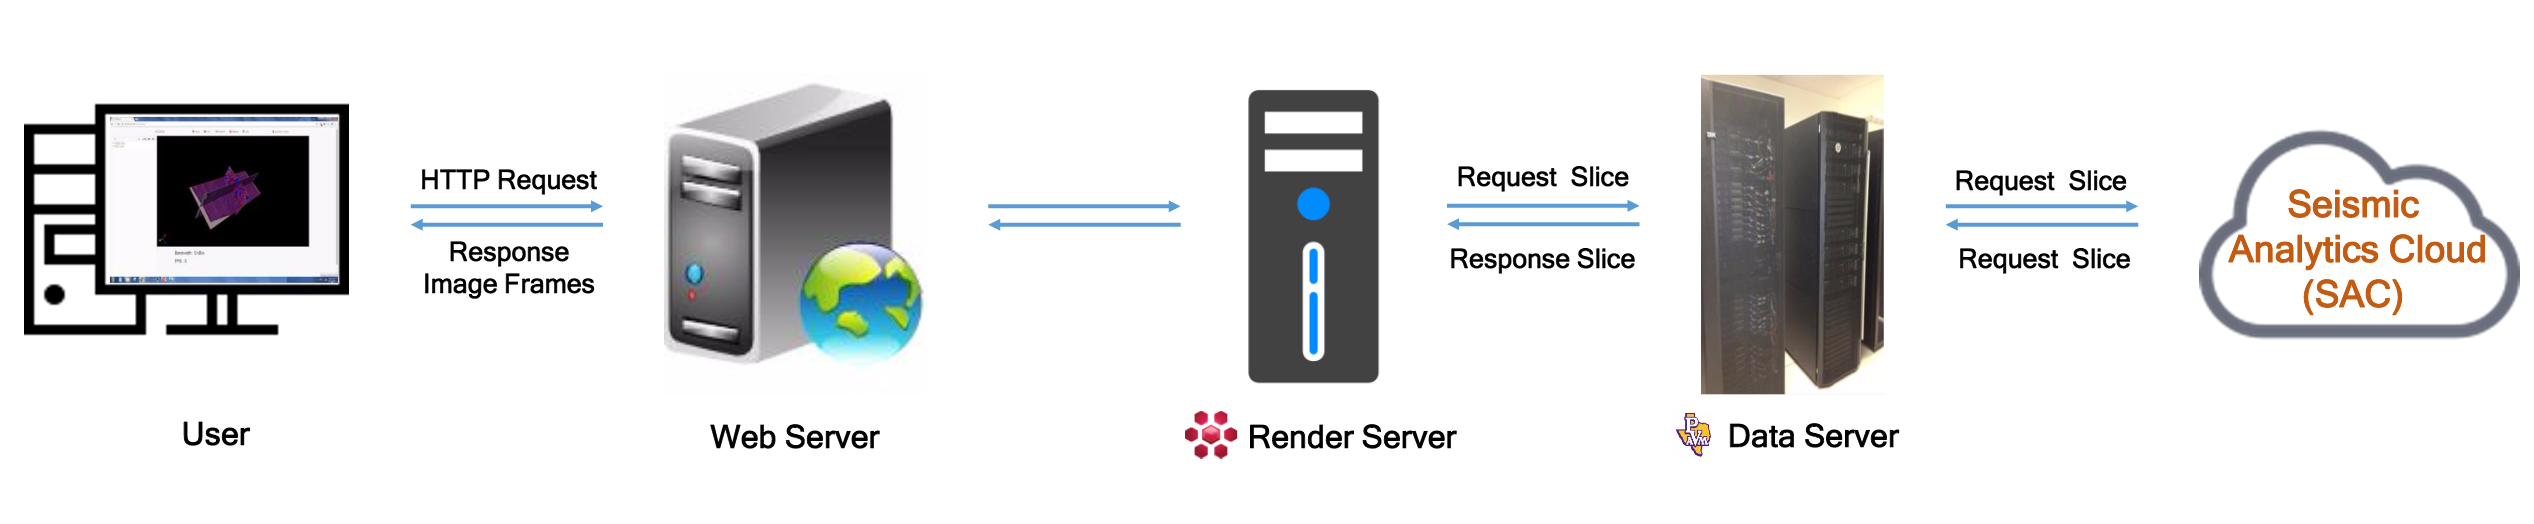
\includegraphics[scale=0.3]{figures/visualization_framework.png}
\caption{The Framework of Remote Web Visualization Service}
\label{visualization_framework}
\end{figure}

This solution is developed on top of Seismic Data Analytics SDK APIs and FEI Digital Rock Visualization Packages. We design and implement the DataServer service on top of Seismic Data Analytics SDK, which could load big seismic datasets from HDFS, transpose and store them to SeismicRDD in backends then feed the requested data in any direction to FEI visualization service in real-time. The FEI Digital Rock Visualization package is developed by FEI, the company which has been focus on featuring Digital Rock technology and solutions many years \cite{FEICompany}. 

Finally, the output rendered data view is presented through web interface and allows user to browse and manipulate in any direction. With this solution, user do not need to install complicated visualization tools and packages since the platform handles everything on server-side. More importantly, the performance of rendering big seismic data is improved and scalable after facilitated by Seismic Data Analytics SDK. Figure \ref{visualization} show s the web interface of this solution.

\begin{figure}[h]
\centering
\includegraphics[scale=0.3]{figures/visualization.png}
\caption{Visualization Web Interface}
\label{visualization}
\end{figure}


\section{Web-based Workflow Platform}

Another service we developed is a web-based workflow platform, which provides a user-friendly web interface to make cloud platform easy to use without programming, with which users could create workflow with drag and drop, could run the pre-built workflow and browse the results via the visualization service. This workflow web service is developed on top of the open-source project Clowdflows \cite{Clowdflows}, which provides a Django based web application framework to develop and manage customized widgets and workflows conveniently. As a free and open source web framework developed in Python, Django follows the classic Model, View and Controller (MVC) architectural pattern, so this application is suitable for interacting with both cloud service and web client.

The client side view of workflow is shown as Figure \ref{workflow}. Users could select widgets and specify seismic data files as input to construct their workflows. Each widget in the workflow view is an independent application component which could be implemented on top of Seismic Data Analytics SDK. A widget acquires at least one port as input or output thus multiple widgets are able to be combined to a workflow by multiple pipelines which connect the ports of all widgets. Each pipeline in the workflow view indicates a data communication, which transports data between widgets and drives the execution of whole workflow. The workflow framework implemented by Python code includes Django views (GUI), Django models (widgets data management) and topological sorting algorithm (connections check).  The data files are stored in HDFS of the cloud platform and could be browsed and selected from the navigation trees on the editor page.

\begin{figure}[h]
\centering
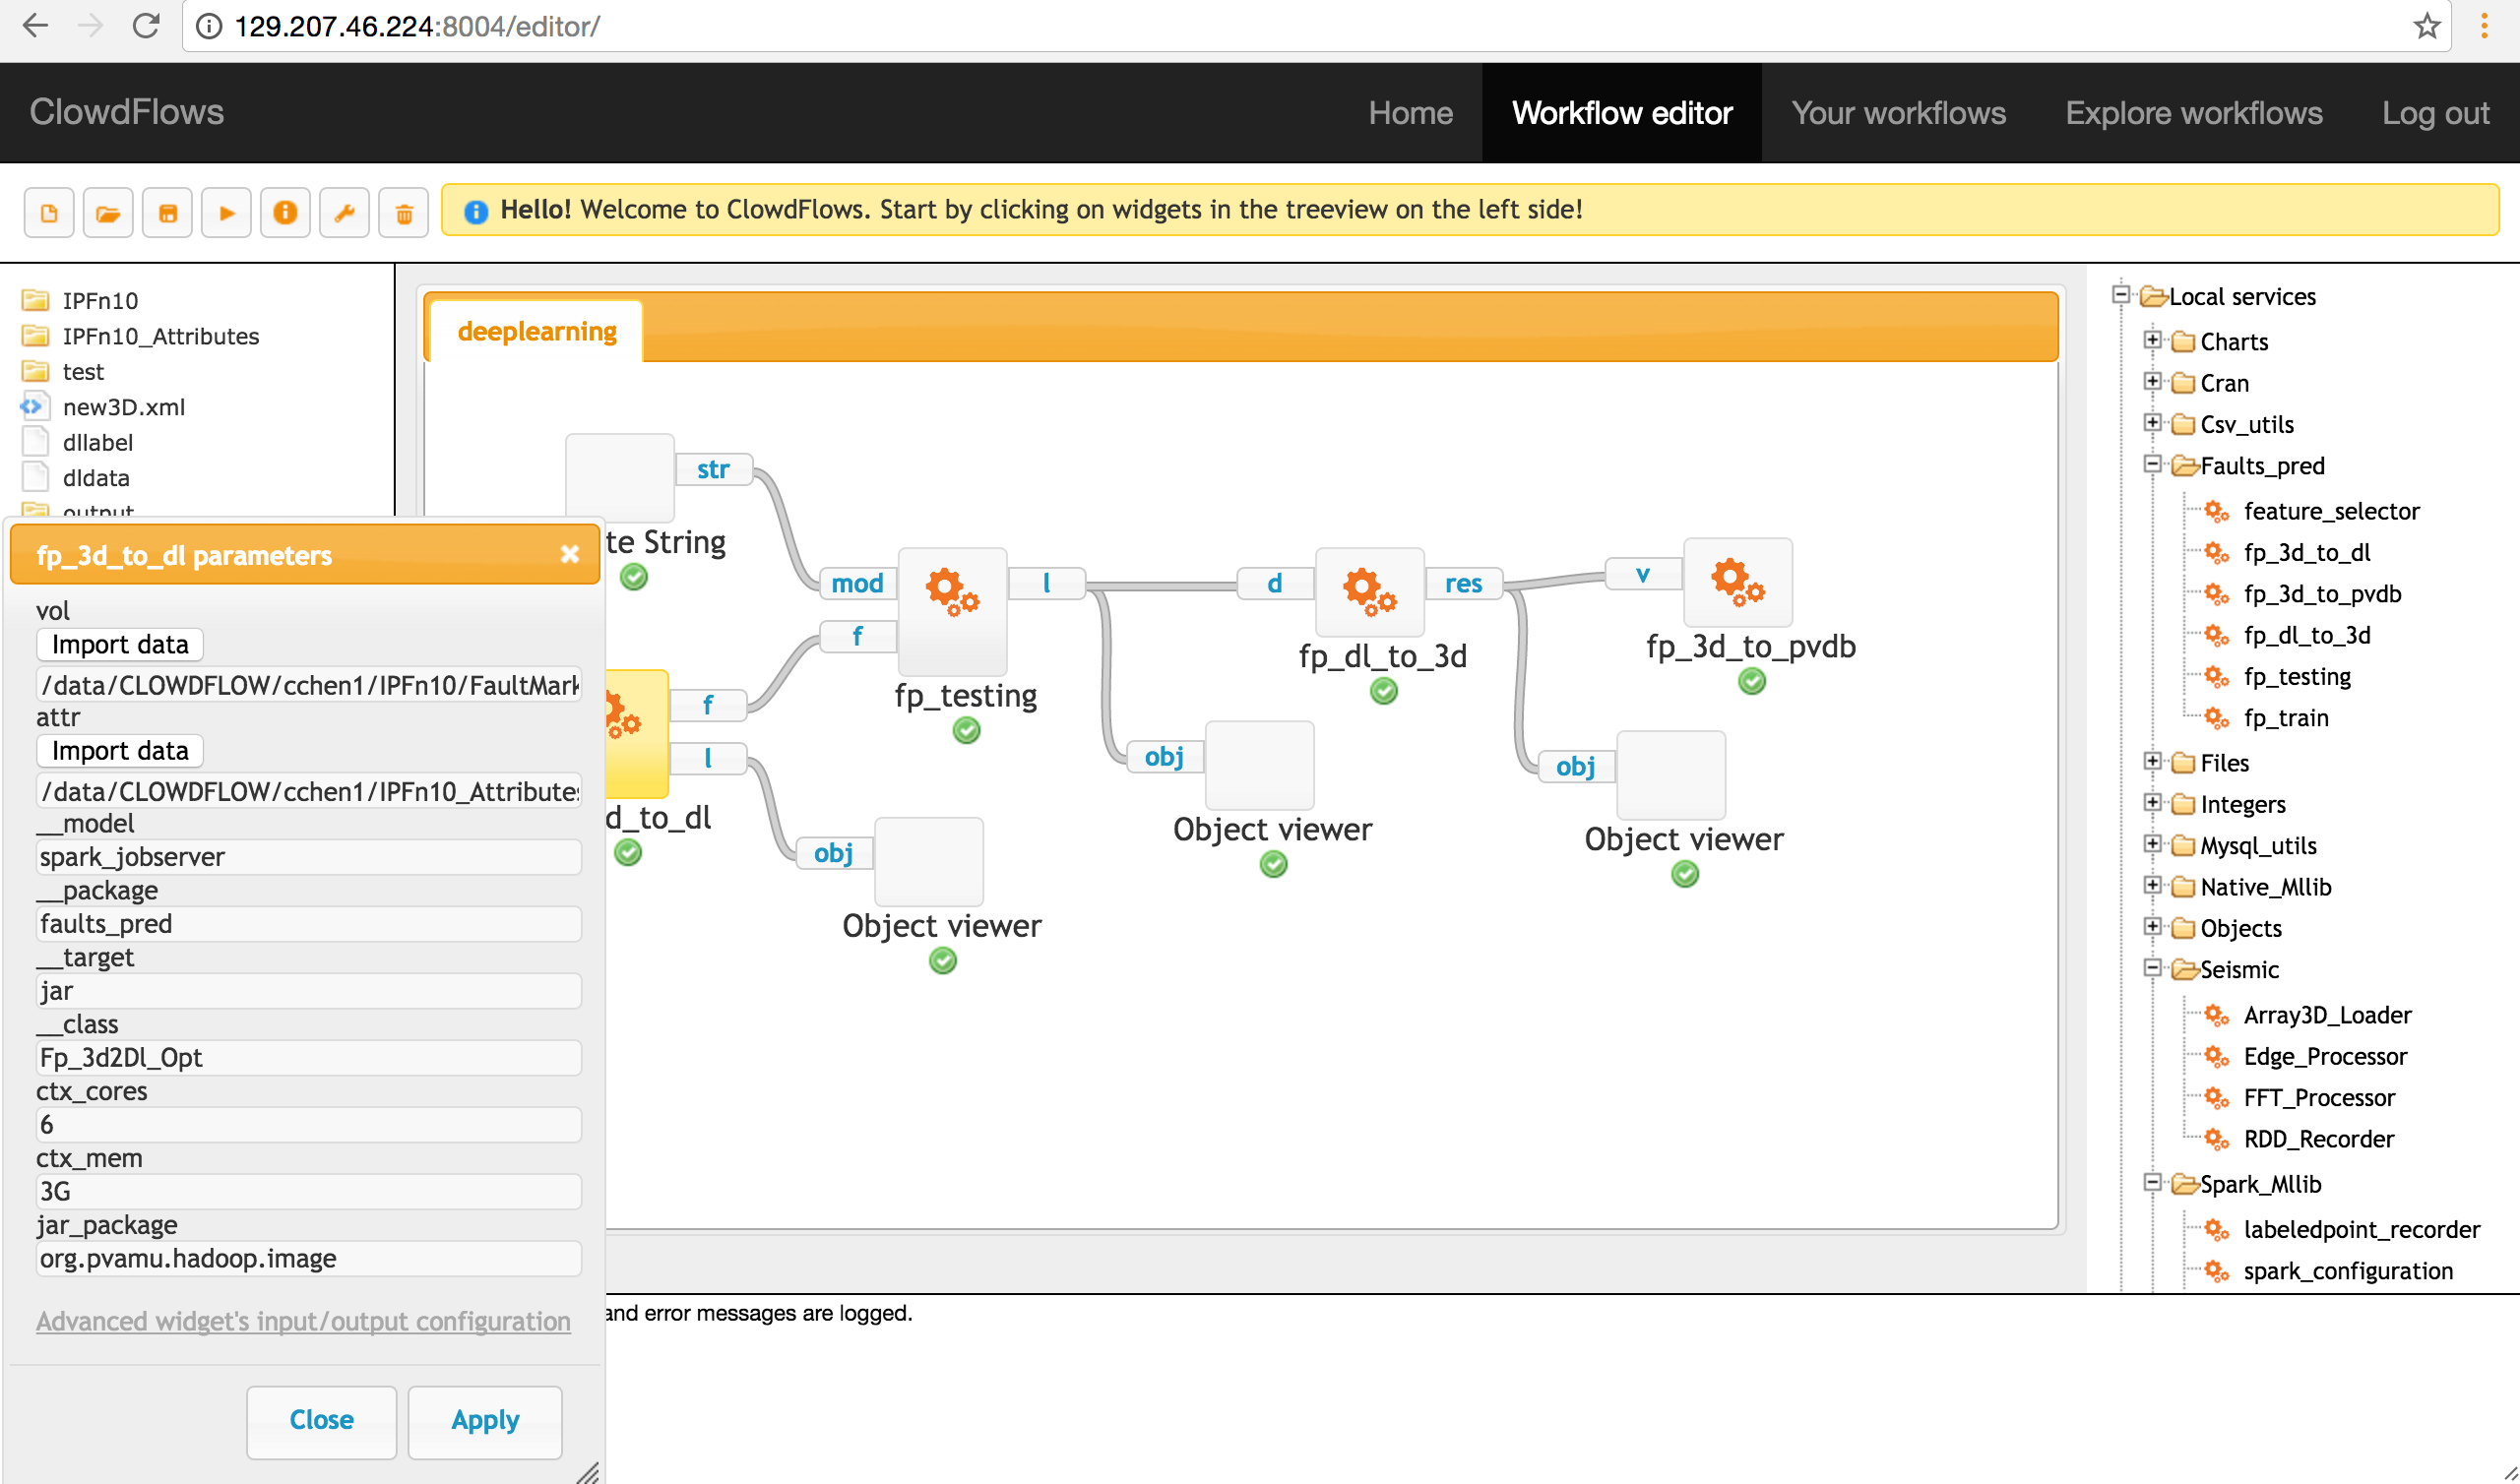
\includegraphics[scale=0.3]{figures/workflow.png}
\caption{Workflow Web Interface}
\label{workflow}
\end{figure}

